
\documentclass[11pt, a4paper]{book}
\usepackage[french]{babel}
\usepackage[utf8]{inputenc}
\usepackage{answers}

\usepackage{hyperref}
\usepackage{multicol}

\usepackage[table,xcdraw]{xcolor}
\usepackage{listings}
\definecolor{ForestGreen}{RGB}{34,139,34}


\usepackage{enumitem}

\AtBeginDocument{\def\labelitemi{$\bullet$}}


\newcommand{\py}{\lstinline{Python} }


\definecolor{backcolour}{rgb}{0.95,0.95,0.92}

\lstset{%
	language         = Python,
	backgroundcolor  = \color{backcolour},
	basicstyle       = \ttfamily, % \upshape\ttfamily,
	keywordstyle     = \bfseries\color{blue}, %\bfseries,
	stringstyle      = \color{magenta},
	commentstyle     = \color{ForestGreen},
	alsoletter = > ,
	morekeywords = {>>>,as,assert,False,None, nonlocal,True, with,yield , <<, >>, :},
	showstringspaces = false,
	numbers=left,
	stepnumber=1,
	literate={à}{{\`{a}}}1 {é}{{\'e}}1 {è}{{\`{e}}}1 {ê}{{\^{e}}}1 {Ê}{{\^{E}}}1 {î}{{\^i}}1 {ô}{{\^{o}}}1 {ç}{{\c{c}}}1 {Ç}{{\c{C}}}1
}

\newcommand{\itemb}[1]{\item \textbf{#1}}

\usepackage{fancyhdr}  %package pour en-tetes et pied de pages
\usepackage{sectsty} % Permet de faire des modifications de police dans diverses sections des "headings" (cf. modif presentation de la page)
\pagestyle{fancy}       %Style pour en-tetes et pieds de pages
\fancyhead[CO,CE]{\sc Série 1\hspace{0.5mm}}
\fancyhead[RO,LE]{Collège Sismondi}  % LaTeX/TEX define \strut to be an invisible box of width zero that extends just enough above and below the baseline. Cela permet d'augementer légèrement la taille en bas de la box de manière à ce qu'elle soit collée à la ligne.
\fancyhead[LO,RE]{\small\ \textsl{1\textsuperscript{ère} année - DO Informatique}}
\fancyfoot[RO,LE]{2021 - 2022}
\fancyfoot[LO,RE]{\small }
\fancyfoot[CO,CE]{\thepage}

\fancyhfoffset[l]{1.2cm} % le "l" en paramètre permet d'indiquer qu'on ne veut modifier que la marge à gauche.
\renewcommand{\headrule}{{%
		\hrule \headwidth \headrulewidth \vskip-\headrulewidth}}
\renewcommand\footrulewidth{\headrulewidth}
\renewcommand{\footrule}{{%
		\vskip-\footruleskip\vskip-\footrulewidth
		\hrule \headwidth \footrulewidth\vskip\footruleskip}}

\usepackage{tikz}
%-------------------------------------------------------------------------------
%---- Eclairage : en encadré sur fond jaune avec symbôle "ampoule" à gauche ----
%-------------------------------------------------------------------------------
\definecolor{coleclairage}{RGB}{255 , 221 , 156}
\definecolor{contoureclairage}{RGB}{255 , 192 , 0}
\newenvironment{eclairage}
{
	\begin{center}%
		\begin{tikzpicture}%
			\node[rectangle, draw=contoureclairage, top color=coleclairage!50, bottom color=coleclairage!140, rounded corners=5pt, inner xsep=5pt, inner ysep=6pt, outer ysep=10pt]\bgroup                     
			\begin{minipage}{0.98\linewidth}
				\begin{minipage}{0.08\linewidth}\centerline{
\includegraphics[scale=1]{Symbole_eclairage.png}}\end{minipage}
				\begin{minipage}{0.89\linewidth}\itshape\footnotesize
				}
				{                		
				\end{minipage}
			\end{minipage}\egroup;%
		\end{tikzpicture}%
	\end{center}%
}

%-------------------------------------------------------------------------------
%---- apprendre : en encadré sur fond jaune avec symbôle "ampoule" à gauche ----
%-------------------------------------------------------------------------------
\definecolor{colapprendre}{RGB}{50,205,50}
\definecolor{contourapprendre}{RGB}{34,139,34}
\newenvironment{apprendre}
{
	\begin{center}%
		\begin{tikzpicture}%
			\node[rectangle, draw=contourapprendre, top color=colapprendre!10, bottom color=colapprendre!50, rounded corners=5pt, inner xsep=5pt, inner ysep=6pt, outer ysep=10pt]\bgroup                     
			\begin{minipage}{0.98\linewidth}
				\begin{minipage}{0.08\linewidth}\centerline{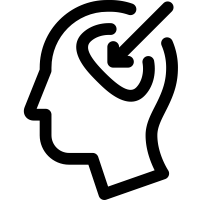
\includegraphics[width=30px]{Symbole_learn.png}}\end{minipage}
				\begin{minipage}{0.89\linewidth}\itshape\footnotesize
				}
				{                		
				\end{minipage}
			\end{minipage}\egroup;%
		\end{tikzpicture}%
	\end{center}%
}

\definecolor{colimportant}{RGB}{247 , 189 , 164}
\definecolor{contourimportant}{RGB}{237 , 125 , 49}
\newenvironment{important}
{
	\begin{center}%
		\begin{tikzpicture}%
			\node[rectangle, draw=contourimportant, top color=colimportant!50, bottom color=colimportant!140, rounded corners=5pt, inner xsep=5pt, inner ysep=6pt, outer ysep=10pt]\bgroup                     
			\begin{minipage}{0.08\linewidth}\centerline{
\includegraphics[scale=0.8]{Symbole_attention.png}}\end{minipage}
			\begin{minipage}{0.89\linewidth}
			}
			{                		
			\end{minipage}\egroup;
		\end{tikzpicture}%
	\end{center}%
}

%-----------------------------------------------------------------
%---- Modification présentation de la page: marges de la page ----
%-----------------------------------------------------------------
%\addtolength{\hoffset}{-1in}              % 1
%\addtolength{\voffset}{-1in}              % 2
\addtolength{\oddsidemargin}{-0.1 in} % 3
\addtolength{\evensidemargin}{-1in} % 3
\addtolength{\topmargin}{-1in}       % 4
\addtolength{\headheight}{6pt}       % 5
%\addtolength{\headsep}{-0.2cm}           % 6
\setlength{\textheight}{26cm}    % 7
\setlength{\textwidth}{16.5cm}      % 8
\addtolength{\marginparsep}{0pt}      % 9
\setlength{\marginparwidth}{0pt}   % 10
\addtolength{\footskip}{-1mm}           %11

\setlength{\parindent}{0em}% pas d'indentation


% Customiser le nom des sections
\usepackage{titlesec}
\titleformat{\section}[hang]{\Large \bfseries}{Série \thesection:\ }{0pt}{}

\renewcommand{\familydefault}{\sfdefault} % pour avoir des polices san serif

\newtheorem{Exc}{Exercice}
\Newassociation{correction}{Soln}{mycor}
\renewcommand{\Solnlabel}[1]{\bfseries Ex #1 }
\def\exo#1{%
	\futurelet\testchar\MaybeOptArgmyexoo}
\def\MaybeOptArgmyexoo{
	\ifx[\testchar \let\next\OptArgmyexoo
	\else \let\next\NoOptArgmyexoo \fi \next}
\def\OptArgmyexoo[#1]{%
	\begin{Exc}[#1]\normalfont}
	\def\NoOptArgmyexoo{%
		\begin{Exc}\normalfont}
		\newcommand{\finexo}{\end{Exc} \vspace{3mm}}
	\newcommand{\flag}[1]{}
	\newcommand{\entete}[1]

\newcommand{\getexocompteur}{{\the\numexpr \arabic{Exc}  \relax}}	
	
\newcommand{\eexo}{\vspace{5mm}} % espace pour séparer les exercices
\pgfplotsset{compat=1.17}
\begin{document}
\chapter{Représentation numérique de l’information}

{\it Objectifs :}
\begin{itemize}
\item Comprendre les différentes manières d'encodage;
\item Distinguer les avantages et les inconvénients de ces encodages

\end{itemize}

\section{Introduction}

Lorsque nous utilisons un logiciel, chaque action que nous effectuons avec la souris ou le clavier par exemple est traduite en langage informatique puis exécutée par l’ordinateur. 

{\it “Transmettre des informations sous forme numérique suppose entre autres d'optimiser la taille des messages transmis pour éviter de surcharger les canaux de transmission, d'être capable de rectifier des erreurs apparues en cours de transmission, de crypter les contenus et d'authentifier les émissaires et les destinataires…” }(Dunod, 2006)

Les images, le son, le texte et les vidéos sont des informations qu’un ordinateur peut traiter. Un ordinateur est composé de circuits électroniques qui fonctionnent à l'électricité. L’information est représentée physiquement par un signal électrique ou magnétique qui, au-delà d'un certain seuil, correspond à la valeur 1 si non par 0. Par conséquent, l’information est toujours sous forme d’un ensemble de nombres écrit en base 2 par exemple 011001.
En 1939, Claude Shannon a été le premier à faire un parallèle entre l'algèbre booléenne (une algèbre binaire, n'acceptant que vrai et faux comme valeurs, et trois fonctions logiques “Et (*), Ou(+), Non(-)”) et le fonctionnement des circuits électriques. Le vrai/faux se transforme en 1 : le courant passe, 0 : il ne passe pas. C'est Shannon qui popularise le terme de bit:

\begin{defi}
Le terme {\bf bit} (b minuscule dans les notations) signifie {\it binary digit }, c'est-à-dire 0 ou 1 en numérotation binaire. Il s'agit de la plus petite unité d'information manipulable par une machine numérique. 


L'{\bf octet} (en anglais {\bf byte} ou B majuscule dans les notations) est une unité d'information composée de 8 bits. Il permet par exemple de stocker un caractère comme une lettre ou un chiffre.
\end{defi}

D'autres termes sont aussi utilisés pour définir certaines longueurs de nombre:
\begin{itemize}
\item Une unité d'information composée de 16 bits est généralement appelée {\bf mot} (en anglais {\bf word}).

\item Une unité d'information de 32 bits de longueur est appelée {\bf mot double} (en anglais {\bf double word}, d'où l'appellation dword).
\end{itemize}

Jusqu'en 1998; 1024 octets valaient 1 kilooctet. Et depuis les nouvelles unités standardisées par l'organisme international IEC sont les suivantes :
\begin{itemize}
\item Un kilooctet (ko) = $10^3$ octets
\item Un mégaoctet (Mo) = $10^6$ octets
\item Un gigaoctet (Go) = $10^9$ octets
\item Un téraoctet (To) = $10^{12}$ octets
\item Un pétaoctet (Po) = $10^{15}$ octets
\item Un exaoctet (Eo) = $10^{18}$ octets
\item Un zettaoctet (Zo) = $10^{21}$ octets
\item Un yottaoctet (Yo) = $10^{24}$ octets
\end{itemize}

\begin{remarque}
Un mégaoctet devrait en principe valoir 1000 x 1000 octets, c'est-à-dire 1'000'000 d'octets, mais il vaut 1024 x 1024 octets en informatique, c'est-à-dire 1'048'576 octets... ce qui correspond à une différence de 4.63 \% !
\end{remarque}

\section{Les bases décimales, binaires et hexadécimales}


\subsection{La base décimale}

Le système décimal (base 10) est celui que nous utilisons dans la vie quotidienne parce que nous avons commencé à compter avec nos doigts. Il comporte 10 symboles de 0 à 9. C'est un système positionnel, c'est-à-dire que l'endroit où se trouve le symbole définit sa valeur.

Par exemple: $(9'875)_{(10)}=9 \cdot 10^3 + 8 \cdot 10^2 + 7\cdot 10^1 + 5 \cdot 10^0$

10 représente la base et les puissances de 0 à 3 le rang de chaque chiffre. Quelle que soit la base, le chiffre de droite est celui des unités. Celui de gauche est celui qui a le poids le plus élevé.

\subsection{Binaire}

Dans les domaines de l'automatisme, de l'électronique et de l'informatique, nous utilisons la base 2. Tous les nombres s'écrivent avec deux chiffres uniquement, 0 et 1.  Car l'algèbre booléenne est à la base de l'électronique numérique. Par exemple, un interrupteur est ouvert ou fermé, une diode électroluminescente (ou LED en anglais) est allumée ou éteinte,  une tension est présente ou absente, un champ magnétique est orienté Nord-Sud ou Sud-Nord.

Le chiffre binaire, qui peut prendre ces deux états, est nommé {\bf Bit} (Binary digit). Les règles sont les mêmes que pour le décimal. 

Par exemple, $1101_{(2)}=1 \cdot 2^3 + 1 \cdot 2^2 + 0 \cdot 2^1 + 1\cdot 2^0=13_{(10)}$ 

\subsubsection{Conversion binaire décimale}

Une autre façon d'obtenir le nombre en base 10, connaissant son écriture en base 2, est d'établir la valeur de chaque chiffre du nombre: celui le plus à droite représente 1, le deuxième représente 2, le troisième représente $2^2=4$, le quatrième représente $2^3=8$...  Par exemple si nous voulons connaitre la valeur décimale du nombre 10 110, nous établissons d'abord une grille avec les différentes puissances de 2:

\begin{center}
\begin{tikzpicture}
	\draw (-1,1) rectangle (0,0) rectangle (1,1) rectangle (2,0) rectangle (3,1) rectangle (4,0) rectangle (5,1) rectangle (6,0);
	\draw (5.5,0.5) node {$1$};
	\draw (4.5,0.5) node {$2$};
	\draw (3.5,0.5) node {$4$};
	\draw (2.5,0.5) node {$8$};
	\draw (1.5,0.5) node {$16$};
	\draw (0.5,0.5) node {$32$};
	\draw (-.5,0.5) node {$64$};
	
\end{tikzpicture}
\end{center}

Ensuite, nous plaçons le nombre en binaire sous cette grille en mettant bien le chiffre des unités sous le carré le plus à droite et nous barrons les cases dont le chiffre associé est 0:

\begin{center}
\begin{tikzpicture}
	\draw (-1,1) rectangle (0,0) rectangle (1,1) rectangle (2,0) rectangle (3,1) rectangle (4,0) rectangle (5,1) rectangle (6,0);
	\draw (5.5,0.5) node {$1$};
	\draw (4.5,0.5) node {$2$};
	\draw (3.5,0.5) node {$4$};
	\draw (2.5,0.5) node {$8$};
	\draw (1.5,0.5) node {$16$};
	\draw (0.5,0.5) node {$32$};
	\draw (-.5,0.5) node {$64$};
	
	\draw (5.5,-0.5) node {$0$};
	\draw (4.5,-0.5) node {$1$};
	\draw (3.5,-0.5) node {$1$};
	\draw (2.5,-0.5) node {$0$};
	\draw (1.5,-0.5) node {$1$};
	\draw (0.5,-0.5) node {$ $};
	\draw (-.5,-0.5) node {$ $};
	
	\draw (-1,0) -- (0,1)
				(0,0) -- (1,1)
				(2,0) -- (3,1)
				(5,0) -- (6,1);
	
\end{tikzpicture}
\end{center}

Il ne reste plus qu'à additionner les nombres qui restent: $16 + 4 + 2=22$

\begin{exercice}
\'Ecrire en base 10 les nombres suivants:
\begin{multicols}{2}
\begin{enumerate}
\item $101_{(2)}$
\item $10 000_{(2)}$
\item $1111_{(2)}$
\item $10101_{(2)}$
\item $10_{(2)}$
\item $111 000_{(2)}$

\end{enumerate}
\end{multicols}
\end{exercice}

\subsubsection{Conversion décimale binaire}

Pour trouver l'écriture binaire d'un nombre écrit en base 10, il existe principalement deux méthodes. 


\; 

La première méthode consiste à décomposer le nombre en somme de puissance de 2 et à utiliser la grille précédente. 

Plus concrètement, si nous voulons écrite 99 en binaire. La plus grande puissance de 2 que nous pouvons prendre dans 99 est 64 (128, la suivante, est trop grande). Il reste ensuite: 99-64=35. Dans 35 on peut mettre 32, et il restera 35-33=3. Dans 3 on ne peut ni mettre 16, ni mettre 8, ni mettre 4. On peut mettre 2. Il reste 1. Dans 1 on peut mettre 1. 

Cela signifie que 99=64+32+2+1. Sur notre grille cela donne:

\begin{center}
\begin{tikzpicture}
	\draw (-1,1) rectangle (0,0) rectangle (1,1) rectangle (2,0) rectangle (3,1) rectangle (4,0) rectangle (5,1) rectangle (6,0);
	\draw (5.5,0.5) node {$1$};
	\draw (4.5,0.5) node {$2$};
	\draw (3.5,0.5) node {$4$};
	\draw (2.5,0.5) node {$8$};
	\draw (1.5,0.5) node {$16$};
	\draw (0.5,0.5) node {$32$};
	\draw (-.5,0.5) node {$64$};
	
	\draw (5.5,-0.5) node {$1$};
	\draw (4.5,-0.5) node {$1$};
	\draw (3.5,-0.5) node {$0$};
	\draw (2.5,-0.5) node {$0$};
	\draw (1.5,-0.5) node {$0$};
	\draw (0.5,-0.5) node {$1$};
	\draw (-.5,-0.5) node {$1$};
	
	\draw (1,0) -- +(1,1)
				(2,0) -- +(1,1)
				(3,0) -- +(1,1)
				;
	
\end{tikzpicture}
\end{center}

Donc $99_{(10)}=1100011_{(2)}$.


\;

La deuxième méthode consiste  effectuer des divisions successives par 2. Le nombre en binaire se lira à l'aide des restes des différentes divisions:

\begin{figure}[h]
\begin{center}
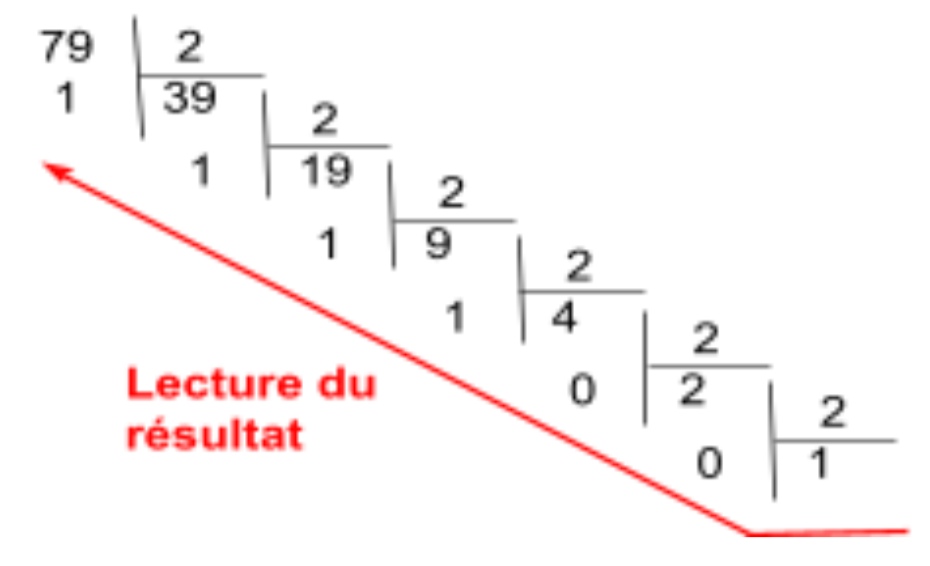
\includegraphics[scale=.5]{images/divisionbinaire}
\end{center}
\end{figure}

Ainsi, $79_{(10)}=1001111_{(2)}$

\begin{exercice}
Les nombres suivants sont écrits en base 10. Donner leur écriture en base 2:
\begin{multicols}{2}
\begin{enumerate}
\item 75
\item 12
\item 27
\item 153
\item 100
\item 200
\item 1000
\item 2000
\end{enumerate}
\end{multicols}
\end{exercice}

\subsection{*La base hexadécimale}

C'est le code utilisé dans la programmation de certains automates et microprocesseurs. Il est composé de : 10 chiffres de 0 à 9, et 6 lettres de A à F. Les adresses MAC (adresses uniques associées à chaque carte réseau dans le monde) sont aussi écrites en base hexadécimale.

La manipulation des nombres écrits en binaire est difficile pour l'être humain et la conversion en décimal n'est pas simple. C'est pourquoi nous utilisons de préférence le système hexadécimal (base 16). 

Le tableau ci-dessous montre la représentation des nombres de 0 à 15 dans les bases 10, 2 et 16.

\begin{figure}[h]
\begin{center}
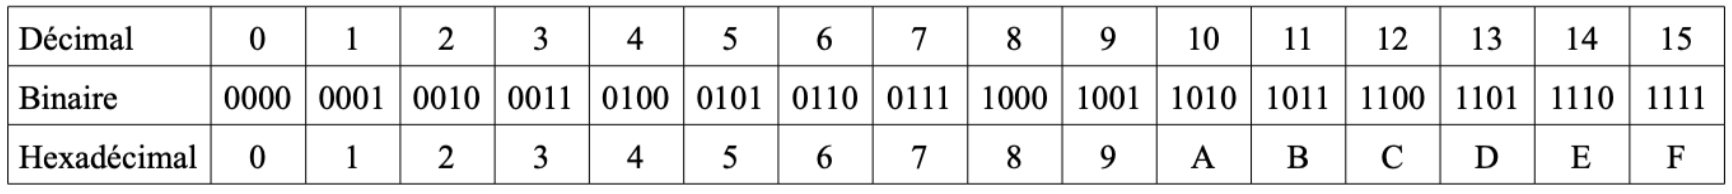
\includegraphics[scale=.5]{images/tableaubase}
\end{center}
\end{figure}


Par exemple, $B4F_{(16)}= B \cdot 16^2 + 4 \cdot 16^1 + F\cdot 16^1= 11 \cdot 16^2 + 4 \cdot 16^1 + 15\cdot 16^0=2 895_{(16)}$

\subsubsection{Conversion en binaire}

Pour convertir un nombre binaire en hexadécimal il suffit de remarquer que chaque groupe de 4 bits représente un chiffre en hexadécimal:

\begin{figure}[h]
\begin{center}
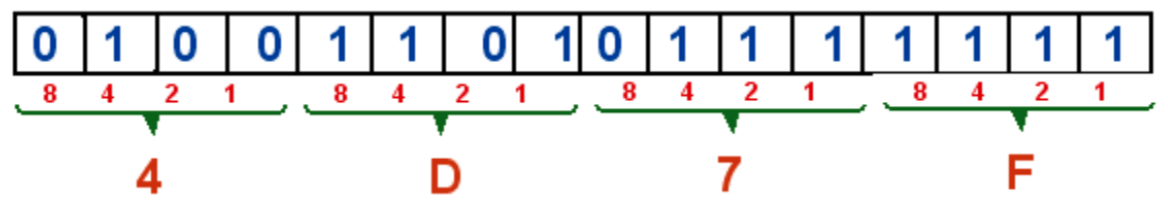
\includegraphics[scale=.5]{images/hexadecimal}
\end{center}
\end{figure}

\begin{exercice}
Écrire les nombres suivants en base hexadécimale:
\begin{multicols}{2}
\begin{enumerate}
\item $10010010110_{(2)}$
\item $111110_{(2)}$
\item  $1000110101110101_{(2)}$
\item $11110000000011_{(2)}$
\end{enumerate}
\end{multicols}
\end{exercice}

\subsubsection{Conversion en décimal}

La méthode par division (par 16) s'applique comme en binaire (par 2).

\begin{exercice}
Écrire les nombres suivants en hexadécimal:
\begin{multicols}{2}
\begin{enumerate}
\item 92
\item 256
\item  500
\item 1023
\end{enumerate}
\end{multicols}
\end{exercice}



\subsection{Opération sur les nombres en binaires}

Tout comme pour l'addition en colonne, pour additionner deux nombres écrits en binaires il faut les additionner bit à bit. 

\begin{exercice}
Quel est le résultat des calculs binaires suivants:
\begin{enumerate}[a)]
\item $0+0=$
\ 

\item $1+0=$
\ 

\item $0+1=$
\ 

\item $1+1=$
\ 

\item $1+1+1=$
\end{enumerate}
\end{exercice}

À l'aide de l'exercice suivant effectué l'addition suivante:

$$1100101001 + 101110101$$

Pour cela, compléter l'addition en colonne suivante:

\;

\begin{center}
\begin{tikzpicture}
	\draw (0,0) node{$1$}
				(0.5,0) node{$1$}
				(1,0) node{$0$}
				(1.5,0) node{$0$}
				(2,0) node{$1$}
				(2.5,0) node{$0$}
				(3,0) node{$1$}
				(3.5,0) node{$0$}
				(4,0) node{$0$}
				(4.5,0) node{$1$};
		\draw (-0.5,-.5) node{$+$}
				(0.5,-.5) node{$1$}
				(1,-.5) node{$0$}
				(1.5,-.5) node{$1$}
				(2,-.5) node{$1$}
				(2.5,-.5) node{$1$}
				(3,-.5) node{$0$}
				(3.5,-.5) node{$1$}
				(4,-.5) node{$0$}
				(4.5,-.5) node{$1$};
	\draw (-1,-.8) -- +(6,0);
\end{tikzpicture}
\end{center}

\vskip+1cm

\begin{exercice}
Effectuer les additions binaires suivantes:
\begin{multicols}{2}
\begin{enumerate}
\item $1001 + 101$
\item $10011 + 110011$
\item  $110001 + 11010$
\item $110101 + 101110$
\end{enumerate}
\end{multicols}
\end{exercice}


\section{Représentation des nombres entiers}

Nous arrivons à écrire tous les nombres entiers naturels en binaire.  Il faut maintenant utiliser un certain nombre de règles pour pouvoir représenter n'importe quel nombre avec un ordinateur: nombres entiers, nombres relatifs, nombres rationnels...

\subsection{Représentation des nombres entiers naturels}

{\it Rappel: Les nombres entiers naturels sont l'ensemble des nombres entiers et positifs. Il est désigné par la lettre $\mathbf{N}=\{0,1,2,\ldots\}$.}

\ 

Nous pouvons par exemple décider que les nombres seront codés sur un octet (8 bits). Le plus petit nombre sera 00000000 = 0 et le plus grand sera 11111111=255.

\, 

{\bf Problème:} En faisant ainsi, nous ne pouvons pas représenter des nombres négatifs.

\subsection{Représentation des nombres entiers relatifs signés}

{\it Rappel: Les nombres entiers  sont l'ensemble des nombres entiers négatifs et positifs. Il est désigné par la lettre $\mathbf{Z}=\{\ldots,-2,-1.0,1,2,\ldots\}$.}

\ 

La première façon pour représenter les nombres négatifs est de décider que le bit le plus gauche représente le signe du nombre.

\begin{figure}[h]
\begin{center}
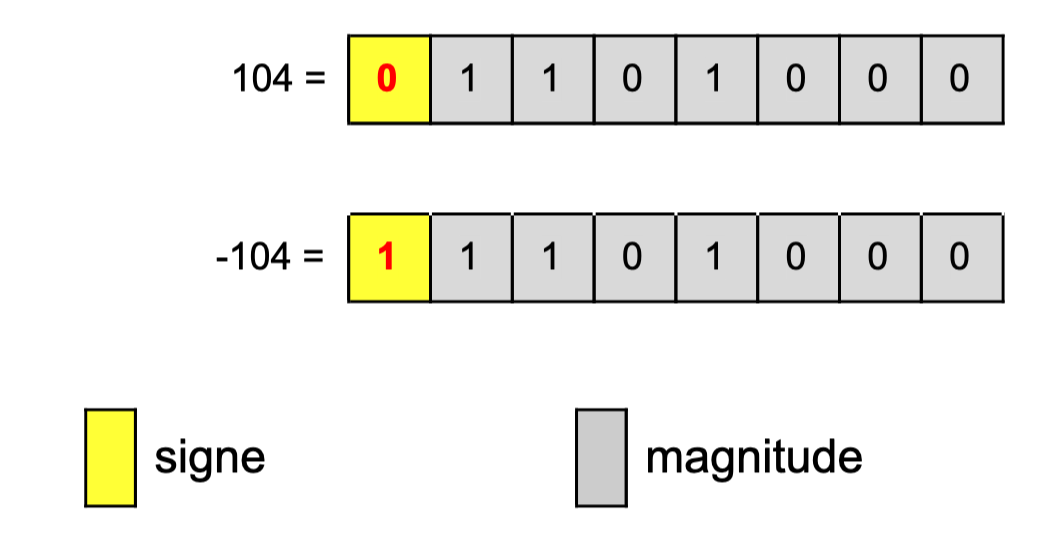
\includegraphics[scale=.5]{images/nombresigne}
\end{center}
\end{figure}

Sur 8 bits plus grand nombre sera 01111111=127 et le plus petit sera 111111111=-127.

\ 

Il est possible d'additionner deux nombres pour autant qu'ils soient tous les deux positifs et que le résultat ne dépasse pas le nombre plus grand nombre pouvant être écrit:

\begin{figure}[h]
\begin{center}
\includegraphics[scale=.5]{images/operationsigne}
\end{center}
\end{figure}

Le résultat de 104 + 30=134 amène un dépassement de capacité. Le nombre entier signé maximum sur 8 bits est 127.


\ 

{\bf Problème:} Bien que pratique, cette façon de coder les nombres négatifs présente deux problèmes:
\begin{enumerate}
\item zéro est représenté de deux façons différentes: 1000000 et 00000000.
\item si on additionne deux nombres opposés, nous n'obtenons pas 0. 
\end{enumerate}

\subsection{* Représentation des nombres en complément à deux}

Cette représentation résout les problèmes de la représentation signée. Dans cette représentation, pour obtenir l'opposé d'un nombre positif écrit en binaire, nous allons effectuer les deux étapes suivantes:
\begin{enumerate}
 \item On inverse tous les bits du nombre positif (on change les 0 en 1 et inversement). Cela s'appelle le {\bf complément à 1}.
 \item On ajoute 1.
\end{enumerate}

Par exemple, nous aimerions écrire le nombre -80. 

Premièrement, 80 s'écrit en binaire: {\bf 01010000}.

\ 

On prend le complément à 1 de ce nombre, ce qui donne: {\bf 10101111}

\ 

Puis on ajoute 1:

\begin{center}
\begin{tikzpicture}
	\draw (0,0) node{$1$}
				(0.5,0) node{$0$}
				(1,0) node{$1$}
				(1.5,0) node{$0$}
				(2,0) node{$1$}
				(2.5,0) node{$1$}
				(3,0) node{$1$}
				(3.5,0) node{$1$};
		\draw (-0.5,-.5) node{$+$}
				
				(3.5,-.5) node{$1$};
				
		
				
	\draw (-1,-.8) -- +(6,0);
	
	\draw  (0,-1.3) node{$1$}
				(0.5,-1.3) node{$0$}
				(1,-1.3) node{$1$}
				(1.5,-1.3) node{$1$}
				(2,-1.3) node{$0$}
				(2.5,-1.3) node{$0$}
				(3,-1.3) node{$0$}
				(3.5,-1.3) node{$0$};
\end{tikzpicture}
\end{center}

L'avantage de cette méthode est que la somme deux nombres opposés donnera bien 0.

\begin{exercice}
En supposant que les nombres soient écrits sur 8 bits, vérifier que 80 + (-80) = 0.
\end{exercice}

\subsection{Résumé}

\begin{figure}[h]
\begin{center}
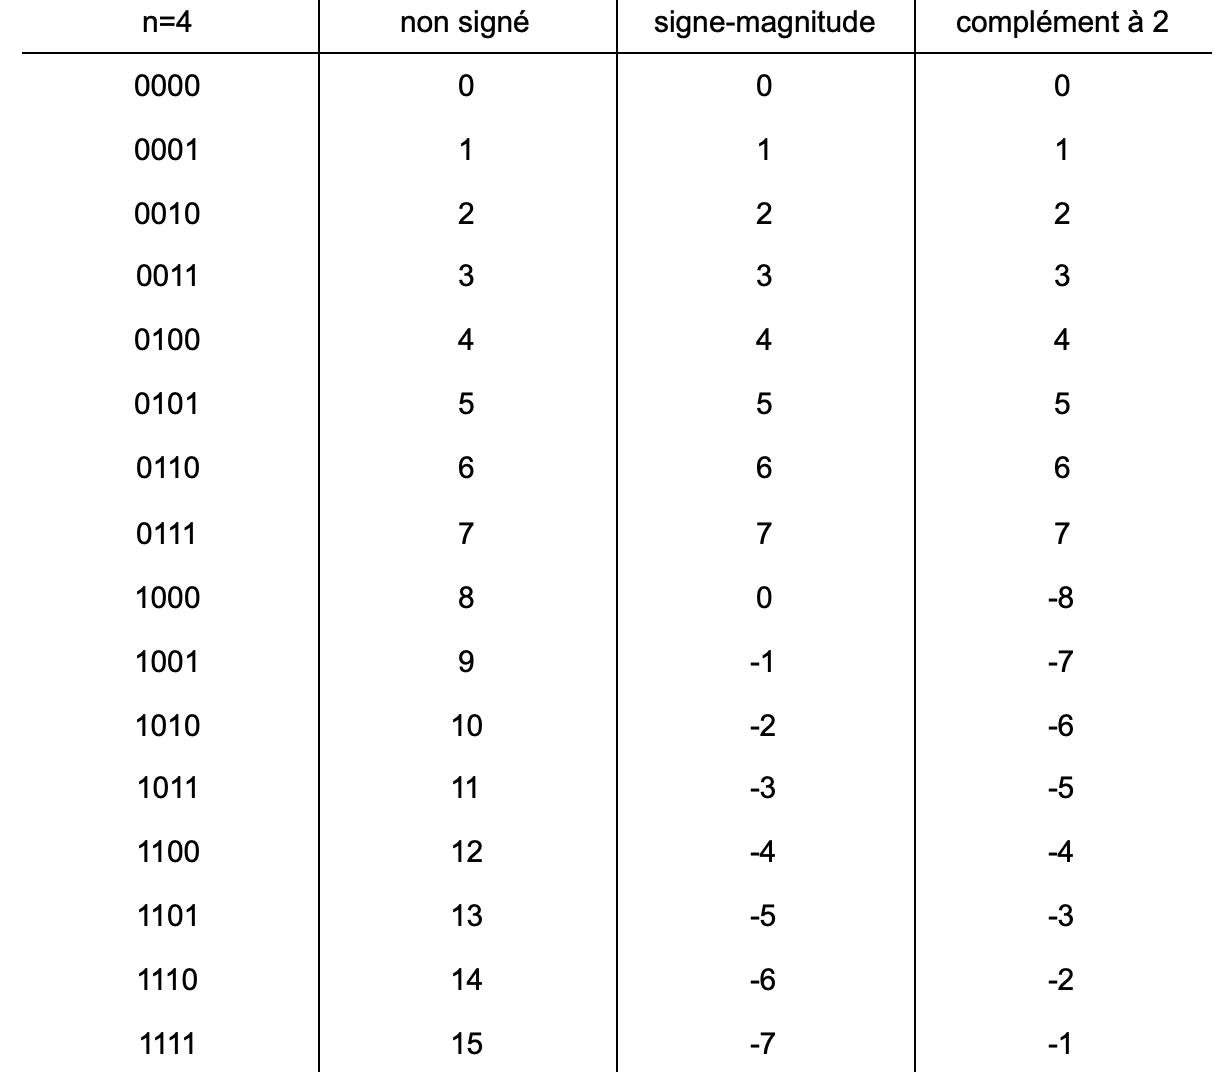
\includegraphics[scale=.55]{images/tablerepresentation}
\end{center}
\end{figure}

\begin{exercice}
Complétez le tableau ci-dessous:



\end{exercice}

\begin{figure}[h]
\begin{center}
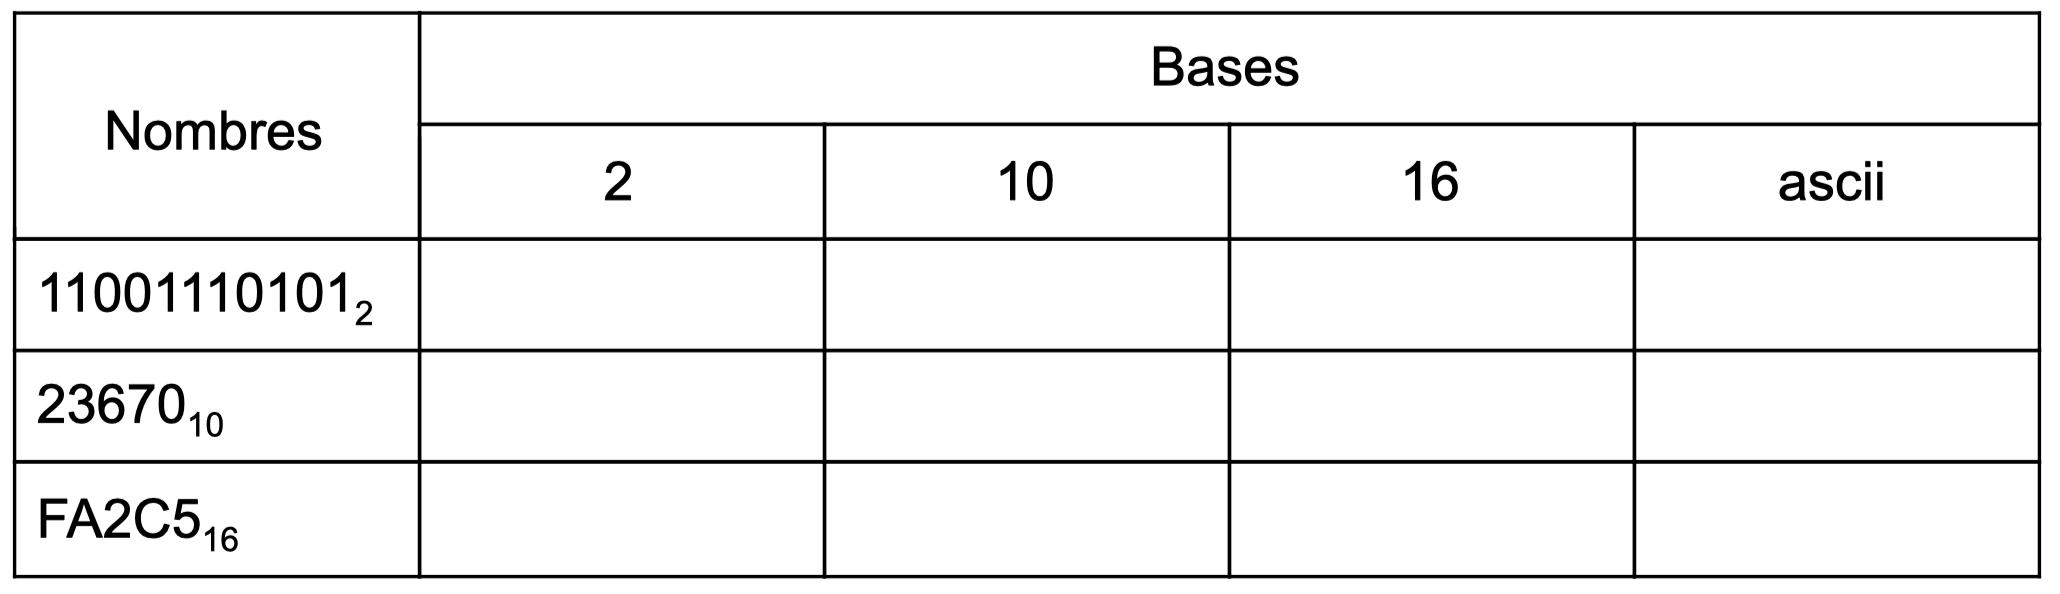
\includegraphics[scale=.3]{images/tableauconversion}
\end{center}
\end{figure}

\begin{exercice}
Utiliser un tableur pour faire une conversion d'une base à l'autre.
\end{exercice}


\begin{exercice}
Donner la représentation signée sur un octet des nombres suivants:
\begin{multicols}{2}
\begin{enumerate}
 	\item -100
 	\item 38
 	\item -200
 	\item -83
\end{enumerate}
\end{multicols}
\end{exercice}


\begin{exercice}*
\begin{enumerate}[a)]
\item Donner la représentation en complément à deux des nombres suivants:

\begin{enumerate}
\item -95
\item -64
\end{enumerate}

\item Vérifier que 95+(-95) donne bien 0 sur un octet.
\item Vérifier que 64+(-6) donne bien 0111010 sur un octet.
\end{enumerate}
\end{exercice}


\begin{exercice}

Nous donnons trois nombres binaires:
\begin{enumerate}[1)]
\item 00101010
\item 1011
\item 10111111
\end{enumerate}

\begin{enumerate}
\item Que valent ces nombres en représentation non signée?
\item * Que valent ces nombres en représentation signée?
\item * Que valent ces nombres en complément à 2?
\end{enumerate}

\end{exercice}

\end{document}